% !TEX root = main.tex

%%%-------------------------------------------
\section*{Листочек 4: алгоритм обратного распространения ошибки}

\addcontentsline{toc}{section}{Листочек 4: алгоритм обратного распространения ошибки}

\epigraph{К толковому выбору приводит опыт,а к нему приводит выбор бестолковый.}{\textit{JSON Стэтхэм}}


%%%-------------------------------------------
\begin{problem}{(граф вычислений)}
    Как найти производную $a$ по $b$ в графе вычислений? Находим не посещённый путь из $a$ в $b$, перемножаем все производные на рёбрах получившегося пути. Добавляем это произведение в сумму. Так делаем для всех путей. Маша хочет попробовать этот алгоритм на функции
    
    $$
    f(x,y) = x^2 + xy + (x + y)^2.
    $$ 
    
    Помогите ей нарисовать граф вычислений и найти $\frac{\partial f}{\partial x}$ и $\frac{\partial f}{\partial y}.$ В каждой вершине графа записывайте результат вычисления одной элементарной операции: сложений или умножения\footnote{По мотивам книги Николенко "Глубокое обучение" (стр. 79)}.
\end{problem} 

\begin{sol}  Нарисуем граф вычислений. 
\begin{center}
    \begin{tikzpicture}
        \tikzstyle{place}=[draw=black,ellipse,minimum height=20pt,minimum width=50pt,inner sep=2pt]
        
        \draw node at (0, 0) [place] (x) {$x$};
        \draw node at (4, 0) [place] (y) {$y$};
        \draw node at (-2, 2) [place] (a) {$a = x^2$};
        \draw node at (1, 2) [place] (b) {$b = x \cdot y$};
        \draw node at (5, 2) [place] (c) {$c = x + y$};
        \draw node at (-1, 4) [place] (d) {$d = a + b$};
        \draw node at (3, 4) [place] (e) {$e = c^2$};
        \draw node at (1, 6) [place] (f) {$f = d + e$};
        
        \draw [->]  (x) to (a);
        \draw [->]  (x) to (b);
        \draw [->]  (x) to (c);
        \draw [->]  (y) to (b);
        \draw [->]  (y) to (c);
        \draw [->]  (a) to (d);
        \draw [->]  (b) to (d);
        \draw [->]  (c) to (e);
        \draw [->]  (e) to (f);
        \draw [->]  (d) to (f);
    \end{tikzpicture}
\end{center}

Каждому ребру припишем производную выхода по входу. Например, ребру между $x$ и $a$ будет соответствовать $\frac{\partial a}{\partial x} = 2x.$

\begin{center}
    \begin{tikzpicture}
        \tikzstyle{place}=[draw=black,ellipse,minimum height=20pt,minimum width=50pt,inner sep=2pt]
        
        \draw node at (0, 0) [place] (x) {$x$};
        \draw node at (4, 0) [place] (y) {$y$};
        \draw node at (-2, 2) [place] (a) {$a = x^2$};
        \draw node at (1, 2) [place] (b) {$b = x \cdot y$};
        \draw node at (5, 2) [place] (c) {$c = x + y$};
        \draw node at (-1, 4) [place] (d) {$d = a + b$};
        \draw node at (3, 4) [place] (e) {$e = c^2$};
        \draw node at (1, 6) [place] (f) {$f = d + e$};
        
        \draw [->, red]  (x) to (a) node[below=1.cm] {$\frac{\partial a}{\partial x} = 2x$};
        \draw [->, red, dashed]  (x) to (b) node[below=10.mm, left] {$\frac{\partial b}{\partial x} = y$};
        \draw [->, amethyst, thick]  (x) to (c) node[below=9mm, left] {$\frac{\partial c}{\partial x} = 1$};
        \draw [->]  (y) to (b) node[below=9.mm, right] {$\frac{\partial b}{\partial y} = x$};
        \draw [->]  (y) to (c) node[below=8.mm, right] {$\frac{\partial c}{\partial y} = 1$};
        \draw [->, red]  (a) to (d) node[below=10.mm, left] {$\frac{\partial d}{\partial a} = 1$};
        \draw [->, red, dashed]  (b) to (d) node[below=10.mm, right] {$\frac{\partial d}{\partial b} = 1$};
        \draw [->, amethyst, thick]  (c) to (e) node[below=10.mm, right] {$\frac{\partial e}{\partial c} = 2c$};
        \draw [->, amethyst, thick]  (e) to (f) node[below=10.mm, right] {$\frac{\partial f}{\partial e} = 1$};
        \draw [->, red]  (d) to (f) node[below=10.mm, left] {$\frac{\partial f}{\partial d} = 1$};
    \end{tikzpicture}
\end{center}

Теперь пройдём по всем траекториям из $x$ в $f$ и перемножим производные на рёбрах. После просуммируем получившиеся множители 

\begin{multline*}
\frac{\partial f}{\partial x} = \frac{\partial f}{\partial d} \cdot \frac{\partial d}{\partial a} \cdot \frac{\partial a}{\partial x} + \frac{\partial f}{\partial d} \cdot \frac{\partial d}{\partial b} \cdot \frac{\partial b}{\partial x} + \frac{\partial f}{\partial e} \cdot \frac{\partial e}{\partial c} \cdot \frac{\partial c}{\partial x} = \\ =  1 \cdot 1 \cdot 2x + 1 \cdot 1 \cdot y + 1 \cdot 2c \cdot 1 = 2x + y + 2(x + y).
\end{multline*}

По аналогии найдём производную по траекториям из $y$ в $f$:

\[
\frac{\partial f}{\partial y} =  1 \cdot 1 \cdot x +  1 \cdot 2c \cdot 1 = x + 2(x + y).
\]
\end{sol} 



%%%-------------------------------------------
\begin{problem}{(придумываем backpropagation)} 
    У Маши есть нейросеть с картинки ниже, где $w_k$ --- веса для $k$ слоя, $f(t)$ --- какая-то функция активации. Маша хочет научиться делать для такой нейронной сетки градиентный спуск.

    \begin{center}
    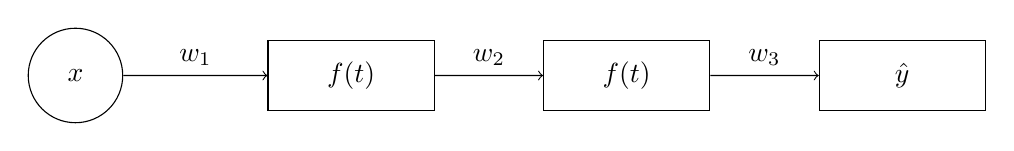
\begin{tikzpicture}[scale=1.4]
    	\tikzstyle{place}=[circle, draw=black, minimum size = 12mm]
    	\tikzstyle{placeh}=[draw=black, minimum height=25pt,minimum width=60pt,inner sep=2pt]
    	
    	% Input
    	\draw node at (0, -2.25) [place] (first) {$x$};
    	\node at (2.5, -2.25) [placeh] (second){$f(t)$};		
    	\node at (5, -2.25) [placeh] (third){$f(t)$};	
    	\node at (7.5, -2.25) [placeh] (fourth){$\hat y$};
    	
    	\draw [->]  (first) to node[above]{$w_1$} (second);
    	\draw [->]  (second) to node[above]{$w_2$} (third);
    	\draw [->]  (third) to node[above]{$w_3$} (fourth);
    \end{tikzpicture}
    \end{center} 
    
    \begin{enumerate}
        \item  Запишите Машину нейросеть, как сложную функцию. 
    	
    	\item Предположим, что Маша решает задачу регрессии. Она прогоняет через нейросетку одно наблюдение. Она вычисляет знчение функции потерь $L(w_1, w_2, w_3) = \frac{1}{2} \cdot (y - \hat y)^2$.  Найдите производные функции $L$ по всем весам $w_k$. 
    	
    	\item В производных постоянно повторяются одни и те же части. Постоянно искать их не очень оптимально. Выделите эти части в прямоугольнички цветными ручками. 
    	
    	\item Выпишите все производные в том виде, в котором их было бы удобно использовать для алгоритма обратного распространения ошибки, а затем, сформулируйте сам алгоритм. Нарисуйте под него удобную схемку.
    \end{enumerate}
\end{problem}

\begin{sol} Чтобы записать нейросеть как сложную функцию, нужно просто последовательно применить все слои

\[
\hat y_i = f(f(f(x_i \cdot w_1) \cdot w_2) \cdot w_3.
\]

Запишем функцию потерь и аккуратно найдём все производные

\[
L(w_1, w_2, w_3) = \frac{1}{2} \cdot (y - \hat y)^2 = \frac{1}{2} \cdot (y - f(f(x \cdot w_1) \cdot w_2) \cdot w_3)^2.
\]

Делаем это по правилу взятия производной сложной функции. Как в школе. 

\begin{equation*}
    \begin{aligned} 
        & \frac{\partial L}{\partial w_3} =  \frac{\partial L}{\partial \hat y} \cdot \frac{\partial \hat y}{\partial w_3} =  (y - \hat{y})  \cdot f(f(x\cdot w_1) \cdot w_2) \\
        & \frac{\partial L}{\partial w_2} =  \frac{\partial L}{\partial \hat y} \cdot \frac{\partial \hat y}{\partial w_2} =  (y - \hat{y}) \cdot  w_3 \cdot f'(f(x\cdot w_1) \cdot w_2) \cdot f(x\cdot w_1) \\
        & \frac{\partial L}{\partial w_1} = \frac{\partial L}{\partial \hat y} \cdot \frac{\partial \hat y}{\partial w_1} =  (y - \hat{y})  \cdot  w_3 \cdot f'(f(x\cdot w_1) \cdot w_2) \cdot w_2 \cdot  f'(x\cdot w_1) \cdot x \\
    \end{aligned} 
\end{equation*}

Выделим в прямоугольники части, которые каждый раз считаются заново, хотя могли бы переиспользоваться. 

\begin{equation*}
    \begin{aligned} 
    & \frac{\partial L}{\partial w_3} =  \frac{\partial L}{\partial \hat y} \cdot \frac{\partial \hat y}{\partial w_3} = \boxed{ (y - \hat{y}) } \cdot f(f(x\cdot w_1) \cdot w_2) \\
    & \frac{\partial L}{\partial w_2} =  \frac{\partial L}{\partial \hat y} \cdot \frac{\partial \hat y}{\partial w_2} = \boxed{ (y - \hat{y})} \cdot \boxed{ w_3 \cdot f'(f(x\cdot w_1) \cdot w_2)} \cdot f(x\cdot w_1) \\
    & \frac{\partial L}{\partial w_1} = \frac{\partial L}{\partial \hat y} \cdot \frac{\partial \hat y}{\partial w_1} = \boxed{ (y - \hat{y}) } \cdot \boxed{ w_3 \cdot f'(f(x\cdot w_1) \cdot w_2)} \cdot w_2 \cdot  f'(x\cdot w_1) \cdot x \\
    \end{aligned} 
\end{equation*}

Если бы слоёв было бы больше, переиспользования возникали бы намного чаще. Градиентный спуск при таком подходе мы могли бы сделать точно также, как и в любых других моделях \begin{equation*}
    \begin{aligned} 
    & w_3^t = w_3^{t-1} - \eta \cdot \frac{\partial L}{\partial w_3}(w_3^{t-1}) \\
    & w_2^t = w_2^{t-1} - \eta \cdot\frac{\partial L}{\partial w_2}(w_2^{t-1}) \\
    & w_1^t = w_1^{t-1} - \eta \cdot\frac{\partial L}{\partial W_1}(w_1^{t-1}).
    \end{aligned} 
\end{equation*}

Проблема в том, что такой подход из-за постоянных перевычислений будет работать долго. Алгоритм обратного распространения ошибки помогает более аккуратно считать производную и ускорить обучение нейросетей. 

Выпишем алгоритм обратного распространения ошибки. Договоримся до следующих обозначений. Буквами $h^k$ будем обозначать выход $k-$го слоя до применения функции активации. Буквами  $o^k$ будем обозначать всё то же самое после применения функции активации. Например, для первого слоя:

\begin{equation*}
    \begin{aligned} 
    & h^1_i = w_1 \cdot x_i \\
    & o^1_i = f(h_i^1). \\
    \end{aligned} 
\end{equation*}

Сначала мы делаем прямой проход по нейросети (forward pass): 

\begin{center}
	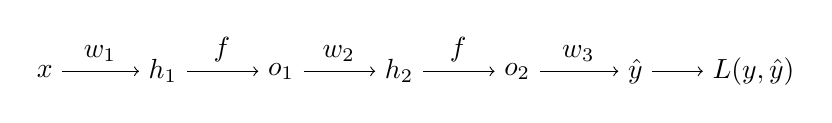
\begin{tikzpicture}
	\tikzstyle{place}=[rectangle, draw=black, minimum size = 8mm]
	\draw node at (0, 0) (input) {$x$};
	\draw node at (1.5, 0) (h1) {$h_1$};
	\draw node at (3, 0) (o1) {$o_1$};
	\draw node at (4.5, 0) (h2) {$h_2$};
	\draw node at (6, 0) (o2) {$o_2$};
	\draw node at (7.5, 0) (output) {$\hat{y}$};
	\draw node at (9, 0) (mse) {$L(y, \hat y)$};
	
	\draw [->]  (input) -- (h1) node[pos=.49, above] {$w_1$} ;
	\draw [->]  (h1) -- (o1) node[pos=.49, above] {$f$} ;
	\draw [->]  (o1) -- (h2) node[pos=.49, above] {$w_2$} ;
	\draw [->]  (h2) -- (o2) node[pos=.49, above] {$f$} ;
	\draw [->]  (o2) -- (output) node[pos=.49, above] {$w_3$} ;
	\draw [->]  (output) to (mse);	
	\end{tikzpicture}
\end{center}

Наша нейросеть --- граф вычислений. Давайте запишем для каждого ребра в рамках этого графа производную. 

\begin{center}
	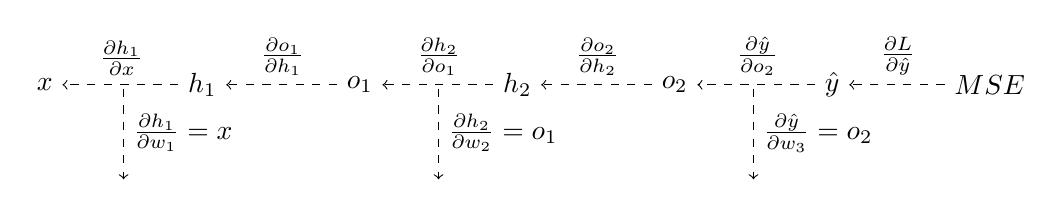
\begin{tikzpicture}
		\draw node at (0, 0) (input) {$x$};
		\draw node at (2, 0) (h1) {$h_1$};
		\draw node at (4, 0) (o1) {$o_1$};
		\draw node at (6, 0) (h2) {$h_2$};
		\draw node at (8, 0) (o2) {$o_2$};
		\draw node at (10, 0) (output) {$\hat{y} $};
		\draw node at (12, 0) (mse) {$MSE$};
		
		\draw [->, dashed]   (h1)  -- (input) node[pos=.49, above] {$\frac{\partial h_1}{\partial x}$} ;
		\draw [->, dashed]   (o1) -- (h1) node[pos=.49, above] {$\frac{\partial o_1}{\partial h_1}$} ;
		\draw [->, dashed]   (h2) -- (o1) node[pos=.49, above] {$\frac{\partial h_2}{\partial o_1}$} ;
		\draw [->, dashed]   (o2) -- (h2) node[pos=.49, above] {$\frac{\partial o_2}{\partial h_2}$} ;
		\draw [->, dashed]   (output) -- (o2)node[pos=.49, above] {$\frac{\partial \hat{y}}{\partial o_2}$} ;
		\draw [->, dashed]  (mse) -- (output) node[pos=.49, above] {$\frac{\partial L}{\partial \hat{y}} $} ;	
		
		\draw [->, dashed]  (9, -0.05) -- (9, -1.2)  node[pos=.49, right] {$\frac{\partial \hat{y}}{\partial w_3} = o_2$} ;
		\draw [->, dashed]  (5, -0.05) -- (5, -1.2)  node[pos=.49, right] {$\frac{\partial h_2}{\partial w_2} = o_1$} ;
		\draw [->, dashed]  (1, -0.05) -- (1, -1.2)  node[pos=.49, right] {$\frac{\partial h_1}{\partial w_1} = x$} ;
	\end{tikzpicture}
\end{center}

Мы везде работаем со скалярами. Все производные довольно просто найти по графу, на котором мы делаем прямой проход. Например,

\[
\frac{\partial h_2}{\partial w_2} = \frac{\partial (o_2 \cdot w_2)}{\partial w_2} = o_2.
\]

Если в качестве функции активации мы используем сигмоиду

\[
f(z) = \sigma(z) = \frac{1}{1 + e^{-z}} = \frac{e^z}{1 + e^{z}},
\]

тогда 

\begin{multline*}
\frac{\partial \sigma }{\partial z} = \left(\frac{e^z}{1 + e^{z}} \right)' = \frac{e^z}{1 + e^{z}} - \frac{e^z}{(1 + e^{z})^2} \cdot e^z  = \frac{e^z}{1 + e^{z}} \left(1 - \frac{e^z}{1 + e^{z}} \right) = \sigma(z)(1 - \sigma(z)).
\end{multline*}

Получается, что 
\[
\frac{\partial o_2}{\partial h_2} = \sigma'(h_2) = \sigma(h_2) \cdot (1 - \sigma(h_2)) = o_2 \cdot (1 - o_2).
\]

Осталось только аккуратно записать алгоритм. В ходе прямого прохода мы запоминаем все промежуточные результаты. Они нам пригодятся для поиска производных при обратном проходе. Например, выше, в сигмоиде, при поиске производной, используется результат прямого прохода $o_2.$

Заведём для накопленного значения производной переменную $d$. На первом шаге нам надо найти $\frac{\partial L}{\partial w_3}$. Сделаем это в два хода

\begin{equation*} 
	\begin{aligned}
		&  d = \frac{\partial L}{\partial \hat y} \\
		&  \frac{\partial L}{\partial w_3} = d \cdot o_2.
	\end{aligned}
\end{equation*}

Для поиска производной $\frac{\partial L}{\partial w_2}$ переиспользуем значение, которое накопилось в $d$. Нам надо найти 

\[
\frac{\partial L}{\partial w_2} = \frac{\partial L}{\hat y} \cdot \frac{\partial \hat y}{\partial o_2} \cdot \frac{\partial o_2}{\partial h_2} \cdot \frac{\partial h_2}{\partial w_2} = d \cdot \boxed{ \frac{\partial \hat y}{\partial o_2} \cdot \frac{\partial o_2}{\partial h_2} } \cdot \frac{\partial h_2}{\partial w_2}.
\]

Часть, выделенную в прямоугольник мы будем переиспользовать для поиска $\frac{\partial L}{\partial w_1}$. Хорошо бы дописать её в $d$ для этого. Получается, вторую производную тоже надо найти в два хода

\begin{equation*} 
	\begin{aligned}
		&  d = d \cdot \frac{\partial \hat y}{\partial o_2} \cdot \frac{\partial o_2}{\partial h_2} \\
		&  \frac{\partial L}{\partial w_2} = d \cdot o_1.
	\end{aligned}
\end{equation*}

Осталась заключительная производная $\frac{\partial L}{\partial w_1}$. Нам надо найти 

\[
\frac{\partial L}{\partial w_2} = \frac{\partial L}{\hat y} \cdot \frac{\partial \hat y}{\partial o_2} \cdot \frac{\partial o_2}{\partial h_2} \cdot \frac{\partial h_2}{\partial o_1} \cdot \frac{\partial o_1}{\partial h_1}  \cdot \frac{\partial h_1}{\partial w_1}  = d \cdot \frac{\partial h_2}{\partial o_1} \cdot \frac{\partial o_1}{\partial h_1}  \cdot \frac{\partial h_1}{\partial w_1}.
\]

Снова делаем это в два шага

\begin{equation*} 
	\begin{aligned}
		&  d = d \cdot  \frac{\partial h_2}{\partial o_1} \cdot \frac{\partial o_1}{\partial h_1} \\
		&  \frac{\partial L}{\partial w_1} = d \cdot x.
	\end{aligned}
\end{equation*}

Если бы нейросетка была бы глубже, мы смогли бы переиспользовать $d$ на следующих слоях. Каждую производную мы нашли ровно один раз. \indef{Это и есть алгоритм обратного распространения ошибки.} В случае матриц происходит всё ровно то же самое, но дополнительно надо проследить за всеми размерностями и более аккуратно перемножить матрицы.
\end{sol} 



%%%-------------------------------------------
\begin{problem}{(сигмоида)}
В \indef{не}глубоких сетях в качестве функции активации можно использовать сигмоиду

\[
\sigma(z) = \frac{1}{1 + e^{-z}} = \frac{e^z}{1 + e^{z}},
\]

Маша хочет использовать сигмоиду внутри нейросети. Предполагается, что после прямого шага, наши вычисления будут использованы в другой части нейросети. В конечном итоге, по выходу из нейросети мы вычислим какую-то функцию потерь $L$. 

У сигмоиды нет параметров. Чтобы обучить нейросеть, Маше понадобится производная $\frac{\partial L}{\partial z}$. Выпишите её в матричном виде через производные $\frac{\partial L}{\partial \sigma}$ и $\frac{\partial \sigma}{\partial z}$.
\end{problem}

\begin{sol} При решении предыдущей задачи мы выяснили, что $\sigma'(z) = \sigma(z) \cdot (1 - \sigma(z)).$ Тогда по цепному правилу 
\[
\frac{\partial L}{\partial z}  = \frac{\partial L}{\partial \sigma} \cdot \frac{\partial \sigma }{\partial z}  =  \frac{\partial L}{\partial \sigma} \cdot \sigma(z) \cdot (1 - \sigma(z)).
\]

Получается, при прямом проходе мы вычисляем сигмоиду по формуле из условия. При обратном проходе мы умножаем пришедшую к нам производную на производную сигмоиды. Если на вход приходит матрица, мы берём сигмоиду от каждого её элемента. Если на вход приходит матрица $Z_{[n \times k]},$ на выходе мы получаем матрицу $\Sigma_{[n \times k]}.$

Когда мы берём сигмоиду от матрицы, мы применяем функцию к каждому её элементу. из-за этого, в производной все умножения мы делаем поэлементно, то есть матрица $\Sigma * (1 - \Sigma)$ останется размера $[n \times k].$  Когда мы применяем цепное правило, под $\frac{\partial L}{\partial \Sigma}$ мы подразумеваем производную функции потерь $L$ по каждому элементу матрицы $\Sigma$. Получается, что это матрица размера $[n \times k].$ Её мы поэлементно умножаем на $\Sigma * (1 - \Sigma)$ и снова получаем матрицу размера $[n \times k].$ Все размерности оказываются соблюдены.
\end{sol} 


%%%-------------------------------------------
\begin{problem}{(линейный слой)}
Маша знает, что главный слой в нейронных сетях --- линейный. В матричном виде его можно записать как $Z = XW.$ 

Маша хочет использовать этот слой внутри нейросети. Предполагается, что после прямого шага наши вычисления будут использованы в другой части нейросети. В конечном итоге, по выходу из нейросети мы вычислим какую-то функцию потерь $L$. 

Чтобы обучить нейросеть, Маше понадобятся производные $\frac{\partial L}{\partial X}$ и $\frac{\partial L}{\partial W}.$  Аккуратно найдите их и запишите в матричном виде\footnote{\url{https://web.eecs.umich.edu/~justincj/teaching/eecs442/notes/linear-backprop.html}}. Предполагается, что 

\[ 
    X = \begin{pmatrix} x_{11} & x_{12} \\  x_{21} & x_{22}  \end{pmatrix} \qquad W  = \begin{pmatrix} w_{11} & w_{12} & w_{13} \\ w_{21} & w_{22} & w_{23}  \end{pmatrix} 
\]\[
	Z = XW = \begin{pmatrix} z_{11} & z_{12} & z_{13}\\  z_{21} & z_{22} & z_{23}  \end{pmatrix} = \begin{pmatrix} x_{11}w_{11} + x_{12}w_{21} & x_{11}w_{12} + x_{12}w_{22} & x_{11}w_{13} + x_{12}w_{23} \\ x_{21}w_{11} + x_{22}w_{21} & x_{21}w_{12} + x_{22}w_{22} & x_{21}w_{13} + x_{22}w_{23} \end{pmatrix}
\]

\end{problem}

\begin{sol} 
При обратном распространении ошибки мы предполагаем, что производная $\frac{\partial L}{\partial Z}$ у нас уже есть. Так как $Z$ --- это матрица размера $2 \times 3,$ эта производная будет выглядеть как 

\[
\frac{\partial L}{\partial Z} = \begin{pmatrix} \frac{\partial L}{\partial z_{11}}  & \frac{\partial L}{\partial z_{12}} & \frac{\partial L}{\partial z_{13}} \\ \frac{\partial L}{\partial z_{21}}  & \frac{\partial L}{\partial z_{22}} & \frac{\partial L}{\partial z_{23}}  \end{pmatrix}.
\]

По цепному правилу мы можем использовать $\frac{\partial L}{\partial Z}$ для поиска интересующих нас градиентов 

\[
\frac{\partial L}{\partial X} = \frac{\partial L}{\partial Z} \cdot \frac{\partial Z}{\partial X} \qquad  \frac{\partial L}{\partial W} = \frac{\partial L}{\partial Z} \cdot \frac{\partial Z}{\partial W}.
\]

Нужно, чтобы у матриц совпали размерности. Производные $\frac{\partial Z}{\partial X}$ и $\frac{\partial Z}{\partial W}$ --- это матрицы Якоби нашего линейного слоя. Пусть $W$ это параметры, а $X$ аргумент функции. Функция $f(X) = XW$ бьёт из пространства матриц $X_{[2 \times 2]}$ в пространство матриц $Z_{[2 \times 3]}$. Нам надо взять производную от каждого элемента матрицы $Z$ по каждому элементу из матрицы $X$. Всего получится $24$ производных. По правилам из матана мы должны будем записать их в виде четырёхмерной матрицы\footnote{Про это можно более подробно почитать в разделе про матричные производные.}. Это жутко неудобно. 

К счастью, многие производные будут нулевыми. Поэтому мы можем схитрить, сначала найти $\frac{\partial L}{\partial X},$ 

\[ 
    X = \begin{pmatrix} x_{11} & x_{12} \\  x_{21} & x_{22}  \end{pmatrix} \quad \Rightarrow \quad  \frac{\partial L}{\partial X} = \begin{pmatrix} \frac{\partial L}{\partial x_{11}}  & \frac{\partial L}{\partial x{12}} \\ \frac{\partial L}{\partial x_{21}}  & \frac{\partial L}{\partial x_{22}}   \end{pmatrix},
\]

а затем написать удобные формулы в общем виде. Найдём $\frac{\partial L}{\partial x_{11}}$ с помощью цепного правила 
\[
\frac{\partial L}{\partial x_{11}} = \sum_{i=1}^n \sum_{j=1}^d \frac{\partial L}{\partial z_{ij}} \cdot \frac{\partial z_{ij}}{\partial x_{11}} = \langle \frac{\partial L}{\partial Z} , \frac{\partial Z}{\partial x_{11}} \rangle.
\]

Работать с суммами неудобно. Мы помним, что $\frac{\partial L}{\partial Z}$ и $\frac{\partial Z}{\partial x_{11}}$ --- матрицы из производных. Поэтому сумму можно записать в виде скалярного произведения матриц. Мы должны в нём умножить элементы матриц друг на друга, а затем сложить.  Давайте найдём производную матрицы $Z$ по $x_{11}$

\[
	Z = XW = \begin{pmatrix} x_{11}w_{11} + x_{12}w_{21} & x_{11}w_{12} + x_{12}w_{22} & x_{11}w_{13} + x_{12}w_{23} \\ x_{21}w_{11} + x_{22}w_{21} & x_{21}w_{12} + x_{22}w_{22} & x_{21}w_{13} + x_{22}w_{23} \end{pmatrix}.
\]

Переменная $x_{11}$ фигурирует только в первой строке

\[
\frac{\partial Z}{\partial x_{11}} = \begin{pmatrix} w_{11} & w_{12}  & w_{13} \\ 0 & 0 & 0 \end{pmatrix}.
\]

Выходит, что 

\[
\frac{\partial L}{\partial x_{11}}  =  \left\langle \begin{pmatrix} \frac{\partial L}{\partial z_{11}}  & \frac{\partial L}{\partial z_{12}} & \frac{\partial L}{\partial z_{13}} \\ \frac{\partial L}{\partial z_{21}}  & \frac{\partial L}{\partial z_{22}} & \frac{\partial L}{\partial z_{23}}  \end{pmatrix} , \begin{pmatrix} w_{11} & w_{12}  & w_{13} \\ 0 & 0 & 0 \end{pmatrix} \right\rangle = \frac{\partial L}{\partial z_{11}} \cdot w_{11} + \frac{\partial L}{\partial z_{12}} \cdot w_{12} +  \frac{\partial L}{\partial z_{13}} \cdot w_{13}.
\]

По аналогии мы можем найти оставшиеся три производные. Например,

\[
\frac{\partial L}{\partial x_{21}}  =  \left\langle \begin{pmatrix} \frac{\partial L}{\partial z_{11}}  & \frac{\partial L}{\partial z_{12}} & \frac{\partial L}{\partial z_{13}} \\ \frac{\partial L}{\partial z_{21}}  & \frac{\partial L}{\partial z_{22}} & \frac{\partial L}{\partial z_{23}}  \end{pmatrix} , \begin{pmatrix} 0 & 0 & 0 \\ w_{11} & w_{12}  & w_{13}  \end{pmatrix} \right\rangle = \frac{\partial L}{\partial z_{21}} \cdot w_{11} + \frac{\partial L}{\partial z_{22}} \cdot w_{12} +  \frac{\partial L}{\partial z_{23}} \cdot w_{13}.
\]

Попробуем выписать $\frac{\partial L}{\partial X}$ через $\frac{\partial L}{\partial Z}$ и $W$

\begin{multline*}
\frac{\partial L}{\partial X} = \begin{pmatrix} \frac{\partial L}{\partial x_{11}}  & \frac{\partial L}{\partial x{12}} \\ \frac{\partial L}{\partial x_{21}}  & \frac{\partial L}{\partial x_{22}}   \end{pmatrix} = \\ = \begin{pmatrix} \frac{\partial L}{\partial z_{11}} \cdot w_{11} + \frac{\partial L}{\partial z_{12}} \cdot w_{12} +  \frac{\partial L}{\partial z_{13}} \cdot w_{13}  &  \frac{\partial L}{\partial z_{11}} \cdot w_{21} + \frac{\partial L}{\partial z_{12}} \cdot w_{22} +  \frac{\partial L}{\partial z_{13}} \cdot w_{23} \\ \frac{\partial L}{\partial z_{21}} \cdot w_{11} + \frac{\partial L}{\partial z_{22}} \cdot w_{12} +  \frac{\partial L}{\partial z_{23}} \cdot w_{13}  &   \frac{\partial L}{\partial z_{21}} \cdot w_{21} + \frac{\partial L}{\partial z_{22}} \cdot w_{22} +  \frac{\partial L}{\partial z_{23}} \cdot w_{23}\end{pmatrix} = \\ = \begin{pmatrix} \frac{\partial L}{\partial z_{11}}  & \frac{\partial L}{\partial z_{12}} & \frac{\partial L}{\partial z_{13}} \\ \frac{\partial L}{\partial z_{21}}  & \frac{\partial L}{\partial z_{22}} & \frac{\partial L}{\partial z_{23}}  \end{pmatrix} \cdot \begin{pmatrix} w_{11} & w_{21} \\ w_{12} & w_{22} \\ w_{13} & w_{23} \end{pmatrix} = \frac{\partial L}{\partial Z} W^T
\end{multline*}

Нам повезло! Наша хитрость увенчалась успехом, и нам удалось записать нашу формулу в виде произведения двух матриц без вычисления четырёхмерных якобианов.

\textbf{Провернём ровно такой же фокус с поиском производной $\frac{\partial L}{\partial W}.$}
\[ 
    W = \begin{pmatrix} w_{11} & w_{12} & w_{13} \\  w_{21} & w_{22} & w_{23}  \end{pmatrix} \quad \Rightarrow \quad  \frac{\partial L}{\partial W} = \begin{pmatrix} \frac{\partial L}{\partial w_{11}}  & \frac{\partial L}{\partial w_{12}} & \frac{\partial L}{\partial w_{13}} \\ \frac{\partial L}{\partial w_{21}}  & \frac{\partial L}{\partial w_{22}}  & \frac{\partial L}{\partial w_{23}}  \end{pmatrix}.
\]

По аналогии с предыдущей производной 
\[
\frac{\partial L}{\partial w_{kl}} = \sum_{i=1}^n \sum_{j=1}^d \frac{\partial L}{\partial z_{ij}} \cdot \frac{\partial z_{ij}}{\partial w_{kl}} = \langle \frac{\partial L}{\partial Z} , \frac{\partial Z}{\partial w_{kl}} \rangle.
\]

По матрице 
\[
	Z = XW = \begin{pmatrix} x_{11}w_{11} + x_{12}w_{21} & x_{11}w_{12} + x_{12}w_{22} & x_{11}w_{13} + x_{12}w_{23} \\ x_{21}w_{11} + x_{22}w_{21} & x_{21}w_{12} + x_{22}w_{22} & x_{21}w_{13} + x_{22}w_{23} \end{pmatrix}
\]

мы можем найти все требуемые производные
\begin{equation*}
    \begin{aligned}
        \frac{\partial Z}{\partial w_{11}} = \begin{pmatrix} x_{11} & 0 & 0 \\ x_{21} & 0 & 0 \end{pmatrix} & \quad \frac{\partial Z}{\partial w_{12}} = \begin{pmatrix} 0 & x_{11} & 0 \\  0 & x_{21} & 0 \end{pmatrix} & \quad \frac{\partial Z}{\partial w_{13}} = \begin{pmatrix} 0  & 0 & x_{11}\\  0  & 0 & x_{21}\end{pmatrix}  \\
        \frac{\partial Z}{\partial w_{21}} = \begin{pmatrix} x_{12} & 0 & 0 \\ x_{22} & 0 & 0 \end{pmatrix}  & \quad  \frac{\partial Z}{\partial w_{22}} = \begin{pmatrix} 0 & x_{12} & 0 \\  0 & x_{22} & 0 \end{pmatrix}  & \quad \frac{\partial Z}{\partial w_{23}} = \begin{pmatrix} 0  & 0 & x_{12}\\  0  & 0 & x_{22}\end{pmatrix}.
    \end{aligned}
\end{equation*}

Чтобы найти $\frac{\partial L}{\partial w_{kl}} $ нам надо посчитать между матрицами $\frac{\partial L}{\partial Z}$ и $\frac{\partial Z}{\partial w_{kl}}$ скалярное произведение. Например,
\[
\frac{\partial L}{\partial w_{21}} =  \left\langle  \begin{pmatrix} \frac{\partial L}{\partial z_{11}}  & \frac{\partial L}{\partial z_{12}} & \frac{\partial L}{\partial z_{13}} \\ \frac{\partial L}{\partial z_{21}}  & \frac{\partial L}{\partial z_{22}}  & \frac{\partial L}{\partial z_{23}}  \end{pmatrix} , \begin{pmatrix} x_{12} & 0 & 0 \\ x_{22} & 0 & 0 \end{pmatrix} \right \rangle = \frac{\partial L}{\partial z_{11}} \cdot x_{12} +   \frac{\partial L}{\partial z_{11}} \cdot x_{22}.
\]

Получается, что всю матрицу $\frac{\partial L}{\partial W}$ целиком можно найти как 
\begin{multline*}
\frac{\partial L}{\partial W} = \frac{\partial L}{\partial W} = \begin{pmatrix} \frac{\partial L}{\partial w_{11}}  & \frac{\partial L}{\partial w_{12}} & \frac{\partial L}{\partial w_{13}} \\ \frac{\partial L}{\partial w_{21}}  & \frac{\partial L}{\partial w_{22}}  & \frac{\partial L}{\partial w_{23}}  \end{pmatrix} = \\ = \begin{pmatrix}  \frac{\partial L}{\partial z_{11}} \cdot x_{11} + \frac{\partial L}{\partial z_{21}} \cdot x_{21} &  \frac{\partial L}{\partial z_{12}} \cdot x_{11} + \frac{\partial L}{\partial z_{22}} \cdot x_{21} & \frac{\partial L}{\partial z_{13}} \cdot x_{11} + \frac{\partial L}{\partial z_{23}} \cdot x_{21} \\ \frac{\partial L}{\partial z_{11}} \cdot x_{12} + \frac{\partial L}{\partial z_{21}} \cdot x_{22} &  \frac{\partial L}{\partial z_{12}} \cdot x_{12} + \frac{\partial L}{\partial z_{22}} \cdot x_{22} & \frac{\partial L}{\partial z_{13}} \cdot x_{12} + \frac{\partial L}{\partial z_{23}} \cdot x_{22} \end{pmatrix}  = \\ =  \begin{pmatrix} x_{11} & x_{21} \\ x_{12} & x_{22} \end{pmatrix} \cdot \begin{pmatrix} \frac{\partial L}{\partial z_{11}}  & \frac{\partial L}{\partial z_{12}} & \frac{\partial L}{\partial z_{13}} \\ \frac{\partial L}{\partial z_{21}}  & \frac{\partial L}{\partial z_{22}} & \frac{\partial L}{\partial z_{23}}  \end{pmatrix} = X^T \frac{\partial L}{\partial Z}.
\end{multline*}

Таким образом, для линейного слоя, мы всегда можем посчитать производные как 
\[
\frac{\partial L}{\partial W}  = X^T \frac{\partial L}{\partial Z} \qquad \frac{\partial L}{\partial X}  = \frac{\partial L}{\partial Z} W^T.
\]

Дальше под $\frac{\partial Z}{\partial W}$ будем всегда подразумевать $X^T,$ а под  $\frac{\partial Z}{\partial X}$ будем иметь в виду $W^T$. 
\end{sol} 



%%%-------------------------------------------------------------------------
\begin{problem}{(Backpropagation в матричном виде)} 
У Маши есть нейросеть с картинки ниже, где $w_{ij}^k$ --- веса для $k$ слоя, $f(t)$ --- какая-то функция активации. Маша хочет научиться делать для такой нейронной сетки градиентный спуск.

    \begin{center}
    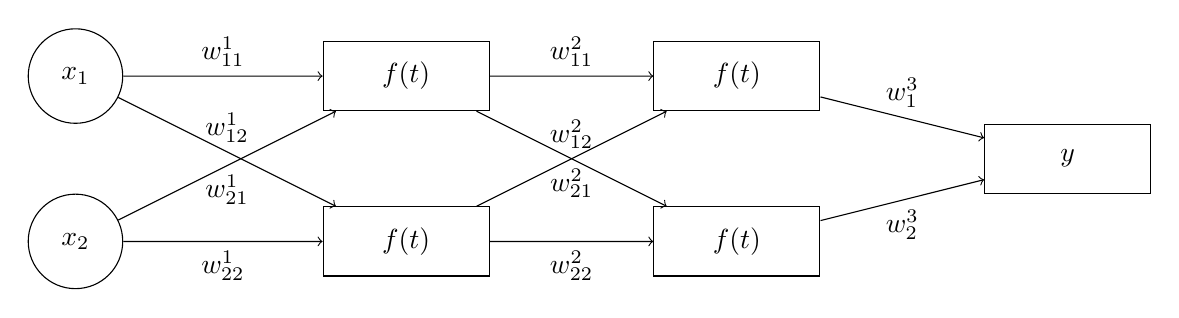
\begin{tikzpicture}[scale=1.4]
    	\tikzstyle{place}=[circle, draw=black, minimum size = 12mm]
    	\tikzstyle{placeh}=[draw=black, minimum height=25pt,minimum width=60pt,inner sep=2pt]
    	
    	% Input
    	\foreach \x in {1,...,2}
    	\draw node at (0, -\x*1.5) [place] (first_\x) {$x_\x$};
    	
    	% Hidden 1
    	\foreach \x in {1,...,2}
    	\node at (3, -\x*1.5) [placeh] (second_\x){$f(t)$};		
    	
    	% Hidden 2
    	\foreach \x in {1,...,2}
    	\node at (6, -\x*1.5) [placeh] (third_\x){$f(t)$};	
    	
    	% Output
    	\node at (9, -2.25) [placeh] (fourth){$y$};
    	
    	\draw [->]  (first_1) to node[above]{$w_{11}^1$} (second_1);
    	\draw [->]  (first_1) to node[above]{$w_{12}^1$} (second_2);
    	\draw [->]  (first_2) to node[below]{$w_{21}^1$} (second_1);
    	\draw [->]  (first_2) to node[below]{$w_{22}^1$} (second_2);
    	
    	\draw [->]  (second_1) to node[above]{$w_{11}^2$} (third_1);
    	\draw [->]  (second_1) to node[above]{$w_{12}^2$} (third_2);
    	\draw [->]  (second_2) to node[below]{$w_{21}^2$} (third_1);
    	\draw [->,]  (second_2) to node[below]{$w_{22}^2$} (third_2);
    	
    	\draw [->]  (third_1) to node[above]{$w_1^3$} (fourth);
    	\draw [->]  (third_2) to node[below]{$w_2^3$} (fourth);
    \end{tikzpicture}
    \end{center} 
    
    \begin{enumerate}
        \item  Запишите Машину нейросеть, как сложную функцию. Сначала в виде нескольких уравнений, а затем в матричном виде. 
    	
    	\item Выпишите все производные в том виде, в котором их было бы удобно использовать для алгоритма обратного распространения ошибки, а затем, сформулируйте сам алгоритм. Нарисуйте под него удобную схемку.
    \end{enumerate}
\end{problem}

\begin{sol} Договоримся до следующих обозначений. Буквами $h^k_{ij}$ будем обозначать выход $k-$го слоя для $j-$го нейрона для $i-$го наблюдения до применения функции активации. Буквами  $o^k_{ij}$ будем обозначать всё то же самое после применения функции активации. Например, для первого слоя:

\begin{equation*}
    \begin{aligned} 
    & h^1_{i1} = w^1_{11} \cdot x_{i1} +  w^1_{21} \cdot x_{i2} \\
    & o^1_{i1} = f(h_{i1}^1). \\
    \end{aligned} 
\end{equation*}

\indef{Делай раз.} Для начала перепишем сетку в виде нескольких уравнений. Для первого слоя мы находим
\begin{equation*}
    \begin{aligned} 
    & o^1_{i1} = f( w^1_{11} \cdot x_{i1} +  w^1_{21} \cdot x_{i2}) \\
    & o^1_{i2} = f( w^1_{12} \cdot x_{i1} +  w^1_{22} \cdot x_{i2}). \\
    \end{aligned} 
\end{equation*}

Для второго работают аналогичные уравнения, но значения $x$ заменяются на соответствующие $o$. На выходе мы предсказываем $y$, как взвешенную суммы выходов со второго слоя
\[
\hat{y}_i = w_1^3 \cdot o^2_{i1} + w_2^3 \cdot o^2_{i2}.
\]

Подставим вместо $o^2_{1i}$ и $o^2_{2i}$ результат вычисления предыдущих слоёв
\[
\hat{y}_i = w_1^3 \cdot f( w^1_{12} \cdot o^1_{i1} +  w^1_{22} \cdot o^1_{i2}) + w_2^3 \cdot f( w^1_{12} \cdot o^1_{i1} +  w^1_{22} \cdot o^1_{i2}).
\]

Подставим результат вычисления первого слоя 
\begin{multline*}
\hat{y}_i = w_1^3 \cdot f( w^1_{12} \cdot f( w^1_{11} \cdot x_{i1} +  w^1_{21} \cdot x_{i2}) +  w^1_{22} \cdot f( w^1_{12} \cdot x_{i1} +  w^1_{22} \cdot x_{i2})) + \\ + w_2^3 \cdot f( w^1_{12} \cdot f( w^1_{11} \cdot x_{i1} +  w^1_{21} \cdot x_{i2}) +  w^1_{22} \cdot f( w^1_{12} \cdot x_{i1} +  w^1_{22} \cdot x_{i2})).
\end{multline*}

Мы записали нашу нейросеть в виде сложной функции. Выглядит ужасно. 

Давайте перепишем всё то же самое более компактно, в матричном виде. Начнём с первого слоя. На самом деле, чтобы найти строчку $(h^1_{i1}, h^1_{i2})$ мы делаем матричное умножение. Строчку $(x_{i1},  x_{i2})$ мы умножаем на матрицу весов $W_1$
\begin{equation*} 
    \begin{pmatrix} h^1_{i1} & h^1_{i2} \end{pmatrix} =  \begin{pmatrix} x_{i1} &  x_{i2}\end{pmatrix} \cdot \begin{pmatrix} w^1_{11} &  w^1_{12} \\ w^1_{21} & w^1_{22}\end{pmatrix}.
\end{equation*} 

Чтобы получить $h_1$ мы умножаем строчку из переменных на первый столбец, чтобы получить $h_2$, на второй столбец. Получается, что в терминах матриц каждый нейрон нашей сети --- это столбец. Если мы добавим ещё один столбец из весов в матрицу, это будет эквивалентно добавлению в сетку третьего нейрона, так как на выходе мы будем получать ещё и $h_3$. Если у нас появится дополнительный вход $x_3$, в матрицу нам нужно будет добавить ещё одну строчку из весов. 

Запишем первый слой в матричном виде. На вход идёт матрица из наблюдений $X_{[n \times 2]}$, она умножается на матрицу весов $W_{[2 \times 2]}$, получается матрица $H_{[n \times 2]}$. Ко всем элементам этой матрицы мы применяем функцию активации $f$. Делаем это поэлементно
\[
O_1 = f(H_1) = f(X\cdot W_1).
\]

Остальные слои записываются по аналогии. Получается, что наша нейросеть в матричном виде выглядит как 
\[
\hat{y} = f(f(X\cdot W_1) \cdot W_2) \cdot W_3.
\]

Здесь $\hat{y}$ --- вектор столбец размера $[n \times 1]$, а матрицы весов обладают размерностями $[2 \times 2]$, $[2 \times 2]$ и $[2 \times 1]$ соответственно. 

\indef{Делай два.} Выпишем алгоритм обратного распространения ошибки в виде красивой схемки. Сначала мы делаем прямой проход по нейросети (forward pass): 

\begin{center}
	\begin{tikzpicture}
	\tikzstyle{place}=[rectangle, draw=black, minimum size = 8mm]
	\draw node at (0, 0) (input) {$\underset{[n \times 2]}{X}$};
	\draw node at (2, 0) (h1) {$\underset{[n \times 2]}{H_1}$};
	\draw node at (4, 0) (o1) {$\underset{[n \times 2]}{O_1}$};
	\draw node at (6, 0) (h2) {$\underset{[n \times 2]}{H_2}$};
	\draw node at (8, 0) (o2) {$\underset{[n \times 2]}{O_2}$};
	\draw node at (10, 0) (output) {$\underset{[n \times 1]}{\hat{y}} $};
	\draw node at (12, 0) (mse) {$L(y, \hat y)$};
	
	\draw [->]  (input) -- (h1) node[pos=.49, above] {$\underset{[2 \times 2]}{W_1}$} ;
	\draw [->]  (h1) -- (o1) node[pos=.49, above] {$f$} ;
	\draw [->]  (o1) -- (h2) node[pos=.49, above] {$\underset{[2 \times 2]}{W_2}$} ;
	\draw [->]  (h2) -- (o2) node[pos=.49, above] {$f$} ;
	\draw [->]  (o2) -- (output) node[pos=.49, above] {$\underset{[2 \times 1]}{W_3}$} ;
	\draw [->]  (output) to (mse);	
	\end{tikzpicture}
\end{center}

Под всеми матрицами подписаны размерности. Взятие функции активации --- поэлементная операция, она никак не меняет размер матрицы. Это будет важно при взятии производных. В ходе прямого прохода мы запоминаем все промежуточные результаты. Они нам пригодятся для поиска производных при обратном проходе. Например, $\frac{\partial H_2}{\partial W_2} = O_1^T.$ Получается, в какой-то момент нам надо будет переиспользовать результаты вычислений, полученных при прямом проходе.

Наша нейросеть --- граф вычислений. Давайте запишем для каждого ребра в рамках этого графа производную. 

\begin{center}
	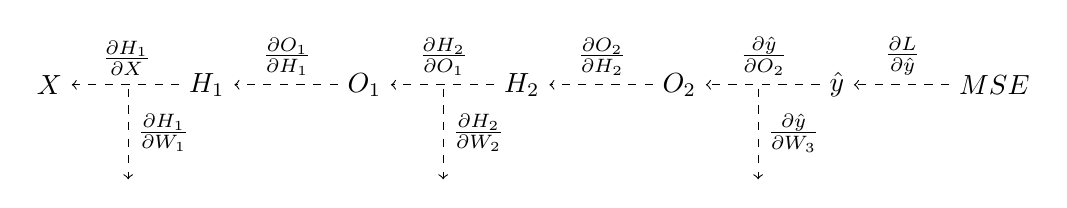
\begin{tikzpicture}
		\draw node at (0, 0) (input) {$X$};
		\draw node at (2, 0) (h1) {$H_1$};
		\draw node at (4, 0) (o1) {$O_1$};
		\draw node at (6, 0) (h2) {$H_2$};
		\draw node at (8, 0) (o2) {$O_2$};
		\draw node at (10, 0) (output) {$\hat{y} $};
		\draw node at (12, 0) (mse) {$MSE$};
		
		\draw [->, dashed]   (h1)  -- (input) node[pos=.49, above] {$\frac{\partial H_1}{\partial X}$} ;
		\draw [->, dashed]   (o1) -- (h1) node[pos=.49, above] {$\frac{\partial O_1}{\partial H_1}$} ;
		\draw [->, dashed]   (h2) -- (o1) node[pos=.49, above] {$\frac{\partial H_2}{\partial O_1}$} ;
		\draw [->, dashed]   (o2) -- (h2) node[pos=.49, above] {$\frac{\partial O_2}{\partial H_2}$} ;
		\draw [->, dashed]   (output) -- (o2)node[pos=.49, above] {$\frac{\partial \hat{y}}{\partial O_2}$} ;
		\draw [->, dashed]  (mse) -- (output) node[pos=.49, above] {$\frac{\partial L}{\partial \hat{y}} $} ;	
		
		\draw [->, dashed]  (9, -0.05) -- (9, -1.2)  node[pos=.49, right] {$\frac{\partial \hat{y}}{\partial W_3}$} ;
		\draw [->, dashed]  (5, -0.05) -- (5, -1.2)  node[pos=.49, right] {$\frac{\partial H_2}{\partial W_2}$} ;
		\draw [->, dashed]  (1, -0.05) -- (1, -1.2)  node[pos=.49, right] {$\frac{\partial H_1}{\partial W_1}$} ;
	\end{tikzpicture}
\end{center}

Осталось только аккуратно записать обратный ход алгоритма. Заведём для накопленного значения производной переменную $d$. На первом шаге нам надо найти $\frac{\partial L}{\partial W_3}$. Не будем забывать, как выглядят производные для линейного слоя, полученные в предыдущей задаче. Сделаем это в два хода

\begin{equation*} 
	\begin{aligned}
		&  d = \frac{\partial L}{\partial \hat y} \\
		&  \frac{\partial L}{\partial W_3} = \frac{\partial L}{\partial \hat y} \cdot \frac{\partial \hat y}{\partial W_3} = O_2^T \cdot d.
	\end{aligned}
\end{equation*}

Матрица $O_2^T$ будет размера $[2 \times n],$ вектор $d$ будет размера $[n \times 1]$, размер производной будет~$[2 \times 1],$ что совпадает с размером матрицы $W_3.$

Для поиска производной $\frac{\partial L}{\partial W_2}$ переиспользуем значение, которое накопилось в $d$

\begin{equation*} 
	\begin{aligned}
		&  d = \frac{\partial L}{\partial H_2} = d \cdot \frac{\partial \hat y}{\partial O_2} \cdot \frac{\partial O_2}{\partial H_2} = d \cdot W_3^T * f'(H_2) \\
		&  \frac{\partial L}{\partial W_2} = O_1^T \cdot d.
	\end{aligned}
\end{equation*}

Размер $d$ был $[n \times 1],$ после персчёта стал $[n \times 1] \cdot [1 \times 2] * [n \times 2] =  [n \times 2].$ Поэлементное умножение на производную функции активации не повлияло на размер матрицы. Размер производной $\frac{\partial L}{\partial W_2}$ оказывается  $[2 \times 2],$ что совпадает с размером матрицы $W_2.$

Осталась заключительная производная $\frac{\partial L}{\partial W_1}$. Нам надо найти 

\begin{equation*} 
	\begin{aligned}
		&  d = \frac{\partial L}{\partial H_1} = \frac{\partial L}{\partial H_2} \cdot  \frac{\partial H_2}{\partial O_1} \cdot \frac{\partial O_1}{\partial H_1} = d \cdot W_2^T * f'(H_1)\\
		&  \frac{\partial L}{\partial W_1} = X^T \cdot d.
	\end{aligned}
\end{equation*}

Если бы сетка была глубже, мы продолжили бы переиспользовать $d$. Каждую производную мы посчитали один раз. Такой алгоритм обучения линеен по числу параметров.
\end{sol} 


%%%-------------------------------------------
\begin{problem}{(Backpropagation своими руками)} 
У Маши есть нейросеть с картинки ниже. Она использует функцию потерь  

\[
L(W_1, W_2, W_3) = \frac{1}{2} \cdot (\hat y - y)^2.
\]

В качестве функции активации Маша выбрала сигмоиду $\sigma(t) = \frac{e^t}{1 + e^t}$.

    \begin{center}
    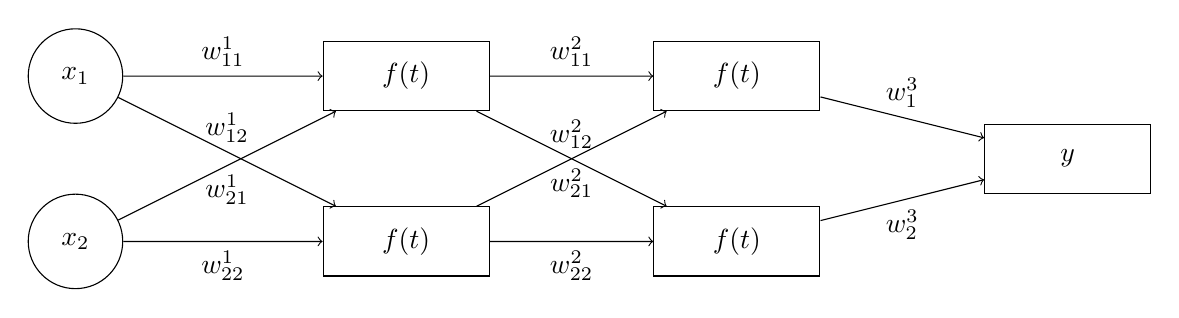
\begin{tikzpicture}[scale=1.4]
    	\tikzstyle{place}=[circle, draw=black, minimum size = 12mm]
    	\tikzstyle{placeh}=[draw=black, minimum height=25pt,minimum width=60pt,inner sep=2pt]
    	
    	% Input
    	\foreach \x in {1,...,2}
    	\draw node at (0, -\x*1.5) [place] (first_\x) {$x_\x$};
    	
    	% Hidden 1
    	\foreach \x in {1,...,2}
    	\node at (3, -\x*1.5) [placeh] (second_\x){$f(t)$};		
    	
    	% Hidden 2
    	\foreach \x in {1,...,2}
    	\node at (6, -\x*1.5) [placeh] (third_\x){$f(t)$};	
    	
    	% Output
    	\node at (9, -2.25) [placeh] (fourth){$y$};
    	
    	\draw [->]  (first_1) to node[above]{$w_{11}^1$} (second_1);
    	\draw [->]  (first_1) to node[above]{$w_{12}^1$} (second_2);
    	\draw [->]  (first_2) to node[below]{$w_{21}^1$} (second_1);
    	\draw [->]  (first_2) to node[below]{$w_{22}^1$} (second_2);
    	
    	\draw [->]  (second_1) to node[above]{$w_{11}^2$} (third_1);
    	\draw [->]  (second_1) to node[above]{$w_{12}^2$} (third_2);
    	\draw [->]  (second_2) to node[below]{$w_{21}^2$} (third_1);
    	\draw [->,]  (second_2) to node[below]{$w_{22}^2$} (third_2);
    	
    	\draw [->]  (third_1) to node[above]{$w_1^3$} (fourth);
    	\draw [->]  (third_2) to node[below]{$w_2^3$} (fourth);
    \end{tikzpicture}
    \end{center} 
    
Выпишите для Машиной нейросетки алгоритм обратного распространения ошибки в общем виде. Пусть Маша инициализировала веса нейронной сети нулями. У неё есть два наблюдения 

\begin{center}
\begin{tabular}{c|c|c|c}
№    &  $x_1$  &  $x_2$  &  $y$ \\ \hline
$1$  &  $1$    &  $1$    &  $1$ \\ 
$2$  &  $5$    &  $2$    &  $0$ \\ 
\end{tabular}
\end{center}

Сделайте руками два шага алгоритма обратного распространения ошибки. Пусть скорость обучения $\eta = 1$. Стохастический градиентный спуск решил, что сначала для шага будет использоваться второе наблюдение, а затем первое. Объясните, почему инициализировать веса нулями --- плохая идея. Почему делать инициализацию весов любой другой константой --- плохая идея? 
\end{problem}

\begin{sol}  Для начала запишем алгоритм в общем виде. Для этого нам надо взять схему из предыдущей задачи и записать там все производные. Для сигмоиды $\sigma'(t) = \sigma(t) \cdot (1 - \sigma(t)).$ Прямой проход по нейронной сети (forward pass):

\begin{center}
	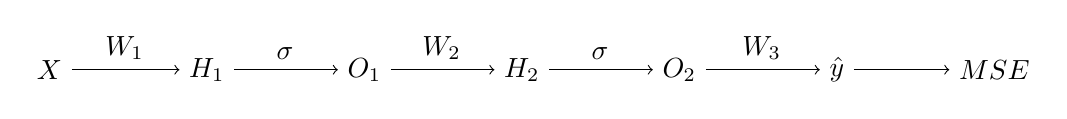
\begin{tikzpicture}
	\tikzstyle{place}=[rectangle, draw=black, minimum size = 8mm]
	\draw node at (0, 0) (input) {$X$};
	\draw node at (2, 0) (h1) {$H_1$};
	\draw node at (4, 0) (o1) {$O_1$};
	\draw node at (6, 0) (h2) {$H_2$};
	\draw node at (8, 0) (o2) {$O_2$};
	\draw node at (10, 0) (output) {$\hat{y} $};
	\draw node at (12, 0) (mse) {$MSE$};
	
	\draw [->]  (input) -- (h1) node[pos=.49, above] {$W_1$} ;
	\draw [->]  (h1) -- (o1) node[pos=.49, above] {$\sigma$} ;
	\draw [->]  (o1) -- (h2) node[pos=.49, above] {$W_2$} ;
	\draw [->]  (h2) -- (o2) node[pos=.49, above] {$\sigma$} ;
	\draw [->]  (o2) -- (output) node[pos=.49, above] {$W_3$} ;
	\draw [->]  (output) to (mse);	
	\end{tikzpicture}
\end{center}

Обратный проход по нейронной сети (backward pass):

\begin{center}
	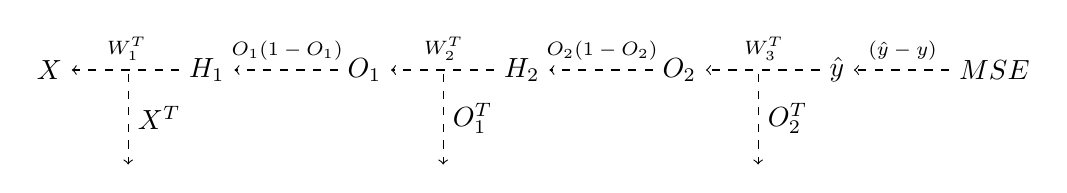
\begin{tikzpicture}
	\draw node at (0, 0) (input) {$X$};
	\draw node at (2, 0) (h1) {$H_1$};
	\draw node at (4, 0) (o1) {$O_1$};
	\draw node at (6, 0) (h2) {$H_2$};
	\draw node at (8, 0) (o2) {$O_2$};
	\draw node at (10, 0) (output) {$\hat{y}$};
	\draw node at (12, 0) (mse) {$MSE$};
	
	\draw [->, dashed]   (h1)  -- (input) node[pos=.49, above] {\scriptsize $W_1^T$} ;
	\draw [->, dashed]   (o1) -- (h1) node[pos=.49, above] {\scriptsize $O_1 (1-O_1)$} ;
	\draw [->, dashed]   (h2) -- (o1) node[pos=.49, above] {\scriptsize $W_2^T$} ;
	\draw [->, dashed]   (o2) -- (h2) node[pos=.49, above] {\scriptsize $O_2 (1 - O_2)$} ;
	\draw [->, dashed]   (output) -- (o2)node[pos=.49, above] {\scriptsize $W_3^T$} ;
	\draw [->, dashed]  (mse) -- (output) node[pos=.49, above] {\scriptsize $(\hat{y} - y)$} ;	
	
	\draw [->, dashed]  (9, -0.05) -- (9, -1.2)  node[pos=.49, right] {$O_2^T$} ;
	\draw [->, dashed]  (5, -0.05) -- (5, -1.2)  node[pos=.49, right] {$O_1^T$} ;
	\draw [->, dashed]  (1, -0.05) -- (1, -1.2)  node[pos=.49, right] {$X^T$} ;
	\end{tikzpicture}
\end{center}

По аналогии с предыдущей задачей выпишем формулы для обратного распространения ошибки:

\begin{minipage}{.2\linewidth}
	\begin{equation*} 
		\begin{aligned}
			&  d = (\hat{y} - y) \\
			&  \frac{\partial MSE}{\partial W_3} = O_2^T \cdot d  \\
		\end{aligned}
	\end{equation*}
\end{minipage} \hfill
\begin{minipage}{.35\linewidth}
	\begin{equation*} 
		\begin{aligned}
			&  d = d \cdot W_3^T * O_2 * (1 - O_2)  \\
			&  \frac{\partial MSE}{\partial W_2} = O_1^T \cdot d \\
		\end{aligned}
	\end{equation*}
\end{minipage} \hfill
\begin{minipage}{.35\linewidth}
	\begin{equation*} 
	\begin{aligned}
	&  d = d \cdot W_2^T * O_1 * (1 - O_1)  \\
	&  \frac{\partial MSE}{\partial W_1} = X^T \cdot d \\
	\end{aligned}
	\end{equation*}
\end{minipage}

Когда мы аккуратно подставим все числа, можно будет сделать шаг SGD

\begin{minipage}{.28\textwidth}
    \[  W_3^t = W_3^{t-1} - \eta \cdot \frac{\partial MSE}{\partial W_3}  \]
\end{minipage}
\begin{minipage}{.3\textwidth}
	\[  W_2^t = W_2^{t-1} - \eta \cdot \frac{\partial MSE}{\partial W_2}  \]
\end{minipage}
\begin{minipage}{.35\textwidth}
	\[  W_1^t = W_1^{t-1} - \eta \cdot \frac{\partial MSE}{\partial W_1}  \]
\end{minipage}

\indef{Сделаем шаг SGD для второго наблюдения.} Делаем прямое распространение для второго наблюдения, напомним, что матрицы весов инициализированы нулями:

\begin{center}
	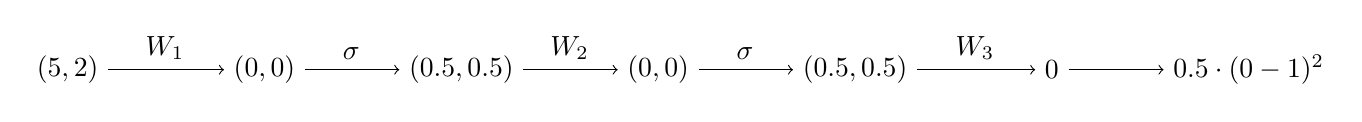
\begin{tikzpicture}
	\tikzstyle{place}=[rectangle, draw=black, minimum size = 8mm]
	\draw node at (0, 0) (input) {$(5, 2)$};
	\draw node at (2.5, 0) (h1) {$(0, 0)$};
	\draw node at (5, 0) (o1) {$(0.5, 0.5)$};
	\draw node at (7.5, 0) (h2) {$(0, 0)$};
	\draw node at (10, 0) (o2) {$(0.5, 0.5)$};
	\draw node at (12.5, 0) (output) {$0$};
	\draw node at (15, 0) (mse) {$0.5 \cdot (0 - 1)^2$};
	
	\draw [->]  (input) -- (h1) node[pos=.49, above] {$W_1$} ;
	\draw [->]  (h1) -- (o1) node[pos=.49, above] {$\sigma$} ;
	\draw [->]  (o1) -- (h2) node[pos=.49, above] {$W_2$} ;
	\draw [->]  (h2) -- (o2) node[pos=.49, above] {$\sigma$} ;
	\draw [->]  (o2) -- (output) node[pos=.49, above] {$W_3$} ;
	\draw [->]  (output) to (mse);	
	\end{tikzpicture}
\end{center}

Делаем обратный проход. 

\textbf{Шаг 1:}
\begin{equation*} 
	\begin{aligned}
		&  d = (\hat{y} - y) = -1 \\
		&  \frac{\partial MSE}{\partial W_3} = O_2^T \cdot  d = \begin{pmatrix} 0.5 \\ 0.5 \end{pmatrix}  \cdot (-1) = \begin{pmatrix} -0.5 \\ -0.5 \end{pmatrix} \\
	\end{aligned}
\end{equation*}
	
\textbf{Шаг 2:}
\begin{equation*} 
	\begin{aligned}
		&  d = d \cdot W_3^T * O_2 * (1 - O_2) = -1 \cdot  (0, 0) * (0.5, 0.5) * (0.5, 0.5) = (0, 0) \\
		&  \frac{\partial MSE}{\partial W_2} = O_1^T \cdot d = \begin{pmatrix} 0.5 \\ 0.5 \end{pmatrix} \cdot (0, 0) = \begin{pmatrix} 0 & 0 \\ 0 & 0 \end{pmatrix} \\
	\end{aligned}
\end{equation*}


\textbf{Шаг 3:}
\begin{equation*} 
	\begin{aligned}
		&  d = d \cdot W_2^T * O_1 * (1 - O_1) = (0, 0) \cdot  \begin{pmatrix} 0 & 0 \\ 0 & 0 \end{pmatrix} * (0.5, 0.5) * (0.5, 0.5) = (0, 0) \\
		&  \frac{\partial MSE}{\partial W_1} = X^T \cdot d = \begin{pmatrix} 5 \\ 2 \end{pmatrix} \cdot (0, 0) = \begin{pmatrix} 0 & 0 \\ 0 & 0 \end{pmatrix} \\
% 		& W_1^1 = \begin{pmatrix} 0 & 0 \\ 0 & 0 \end{pmatrix} - 1 \cdot \begin{pmatrix} 0 & 0 \\ 0 & 0 \end{pmatrix} = \begin{pmatrix} 0 & 0 \\ 0 & 0 \end{pmatrix}
	\end{aligned}
\end{equation*}

Делаем шаг градиентного спуска
\begin{equation*} 
	\begin{aligned}
		& W_1^1 = \begin{pmatrix} 0 & 0 \\ 0 & 0 \end{pmatrix} - 1 \cdot \begin{pmatrix} 0 & 0 \\ 0 & 0 \end{pmatrix} = \begin{pmatrix} 0 & 0 \\ 0 & 0 \end{pmatrix}\\
		& W_2^1 = \begin{pmatrix} 0 & 0 \\ 0 & 0 \end{pmatrix} - 1 \cdot \begin{pmatrix} 0 & 0 \\ 0 & 0 \end{pmatrix} = \begin{pmatrix} 0 & 0 \\ 0 & 0 \end{pmatrix} \\
		& W_3^1 = \begin{pmatrix} 0 \\ 0 \end{pmatrix} - 1 \cdot \begin{pmatrix} -0.5 \\ -0.5 \end{pmatrix} = \begin{pmatrix} 0.5 \\ 0.5 \end{pmatrix}
	\end{aligned}
\end{equation*}

\indef{Сделаем шаг SGD для первого наблюдения.} Делаем прямое распространение для второго наблюдения, напомним, что матрицы весов инициализированы нулями:

\begin{center}
	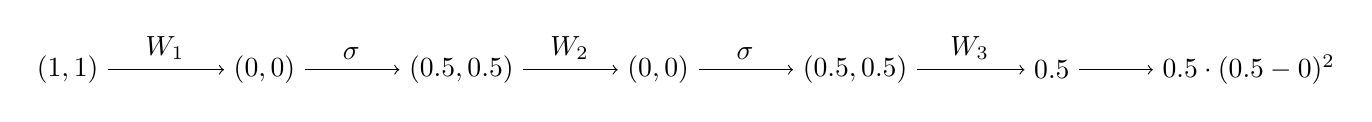
\begin{tikzpicture}
	\tikzstyle{place}=[rectangle, draw=black, minimum size = 8mm]
	\draw node at (0, 0) (input) {$(1, 1)$};
	\draw node at (2.5, 0) (h1) {$(0, 0)$};
	\draw node at (5, 0) (o1) {$(0.5, 0.5)$};
	\draw node at (7.5, 0) (h2) {$(0, 0)$};
	\draw node at (10, 0) (o2) {$(0.5, 0.5)$};
	\draw node at (12.5, 0) (output) {$0.5$};
	\draw node at (15, 0) (mse) {$0.5 \cdot (0.5 - 0)^2$};
	
	\draw [->]  (input) -- (h1) node[pos=.49, above] {$W_1$} ;
	\draw [->]  (h1) -- (o1) node[pos=.49, above] {$\sigma$} ;
	\draw [->]  (o1) -- (h2) node[pos=.49, above] {$W_2$} ;
	\draw [->]  (h2) -- (o2) node[pos=.49, above] {$\sigma$} ;
	\draw [->]  (o2) -- (output) node[pos=.49, above] {$W_3$} ;
	\draw [->]  (output) to (mse);	
	\end{tikzpicture}
\end{center}

Делаем обратный проход. 

\textbf{Шаг 1:}
\begin{equation*} 
	\begin{aligned}
		&  d = (\hat{y} - y) = 0.5 \\
		&  \frac{\partial MSE}{\partial W_3} = O_2^T \cdot  d = \begin{pmatrix} 0.5 \\ 0.5 \end{pmatrix}  \cdot (0.5) = \begin{pmatrix} 0.25 \\ 0.25 \end{pmatrix} \\
	\end{aligned}
\end{equation*}
	
\textbf{Шаг 2:}
\begin{equation*} 
	\begin{aligned}
		&  d = d \cdot W_3^T * O_2 * (1 - O_2) = 0.5 \cdot  (0.5, 0.5) * (0.5, 0.5) * (0.5, 0.5) = (1/16, 1/16) \\
		&  \frac{\partial MSE}{\partial W_2} = O_1^T \cdot d = \begin{pmatrix} 0.5 \\ 0.5 \end{pmatrix} \cdot (1/16, 1/16) = \begin{pmatrix} 1/32 & 1/32 \\ 1/32 & 1/32 \end{pmatrix} \\
	\end{aligned}
\end{equation*}

\textbf{Шаг 3:}
\begin{equation*} 
	\begin{aligned}
		&  d = d \cdot W_2^T * O_1 * (1 - O_1) = (1/16, 1/16) \cdot  \begin{pmatrix} 0 & 0 \\ 0 & 0 \end{pmatrix} * (0.5, 0.5) * (0.5, 0.5) = (0, 0) \\
		&  \frac{\partial MSE}{\partial W_1} = X^T \cdot d = \begin{pmatrix} 1 \\ 1 \end{pmatrix} \cdot (0, 0) = \begin{pmatrix} 0 & 0 \\ 0 & 0 \end{pmatrix} \\
	\end{aligned}
\end{equation*}

На этой задаче видно, как сигмоида способствует затуханию градиента. Её производная по абсолютной величине всегда принимает значения меньше $1$. Из-з этого значение $d$ от слоя к слою становится всё меньше и меньше. Чем ближе к началу нашей сети мы находимся, тем на меньшую величину шагают веса. Если сетка оказывается очень глубокой, такой эффект ломает её обучение. Его обычно называют \indef{параличом нейронной сети.} Именно из-за этого сигмоиду обычно не используют в глубоких архитектурах. 

Делаем шаг градиентного спуска
\begin{equation*} 
	\begin{aligned}
        & W_3^2 = \begin{pmatrix} 0.5 \\ 0.5 \end{pmatrix} - 1 \cdot \begin{pmatrix} 0.25 \\ 0.25 \end{pmatrix} = \begin{pmatrix} 0.25 \\ 0.25 \end{pmatrix} \\
        & W_2^2 = \begin{pmatrix} 0 & 0 \\ 0 & 0 \end{pmatrix} - 1 \cdot \begin{pmatrix}1/32 & 1/32 \\ 1/32 & 1/32 \end{pmatrix} = \begin{pmatrix} -1/32 & -1/32 \\ -1/32 & -1/32 \end{pmatrix} \\
        & W_1^1 = \begin{pmatrix} 0 & 0 \\ 0 & 0 \end{pmatrix} - 1 \cdot \begin{pmatrix} 0 & 0 \\ 0 & 0 \end{pmatrix} = \begin{pmatrix} 0 & 0 \\ 0 & 0 \end{pmatrix}
	\end{aligned}
\end{equation*}

Из-за того, что мы инициализировали веса нулями, слои поначалу учатся по-очереди. Пока мы не сдвинем веса более поздних слоёв, веса более ранних слоёв не сдвинутся. Это замедляет обучение. Обратите внимание, что все веса меняются на одну и ту же величину в одном и том же направлении. При инициализации любой другой константой этот эффект сохраниться. Нам хочется, чтобы после обучения нейроны внутри сетки были максимально разнообразными. Для этого веса лучше инициализировать случайно. В будущем мы обсудим грамотные способы инициализации, которые не портят обучение. 
\end{sol} 


%%%-------------------------------------------
\begin{problem}{(Незаметный backpropagation)}
    Маша собрала нейросеть: 
	
	\begin{equation*}
	y =   \max \left( 0;  X \cdot  \begin{pmatrix} 1 & -1 \\ 0.5 & 0 \end{pmatrix} \right) \cdot \begin{pmatrix} 0.5 \\ 1 \end{pmatrix} 
	\end{equation*}

	Теперь Маша внимательно смотрит на неё.
	
	\begin{enumerate}
		\item[а)]  Первый слой нашей нейросетки --- линейный. По какой формуле делается forward pass? Сделайте его для матрицы \[X =\begin{pmatrix} 1 & 2 \\ -1 & 2 \end{pmatrix}.\] 
		
		\item[б)] Найдите для первого слоя производную выхода по входу. При обратном движении по нейросетке, в первый слой пришёл накопленный градиент \[d = \begin{pmatrix} -0.5 & 0 \\ 0 & 0 \end{pmatrix}.\] Каким будет новое накопленное значение градиента, которое выплюнет из себя линейный слой? По какой формуле делается backward pass? 
		
		\item[в)] Второй слой нейросетки --- функция активации, $ReLU.$  По какой формуле делается forward pass? Сделайте его для матрицы \[H_1 = \begin{pmatrix} 2 & -0.5 \\ 0 & 1 \end{pmatrix}.\]
		
		\item[г)] Найдите для второго слоя производную выхода по входу. При обратном движении по нейросетке во второй слой пришёл накопленный градиент \[d = \begin{pmatrix} -0.5 & -1 \\ 0 & 0 \end{pmatrix}.\]  Каким будет новое накопленное значение градиента, которое выплюнет из себя $ReLU$?  По какой формуле делается backward pass? 
		
		\item[д)] Третий слой нейросетки --- линейный.  По какой формуле делается forward pass? Сделайте его для матрицы \[O_1 =\begin{pmatrix} 2 & 0 \\ 0 & 1 \end{pmatrix}.\]  
		
		\item[е)] Найдите для третьего слоя производную выхода по входу. При обратном движении по нейросетке, в третий слой пришёл накопленный градиент $d = (-1, 0)^T$. Каким будет новое накопленное значение градиента, которое выплюнет из себя линейный слой? 

		\item[ж)] Мы решаем задачу Регрессии. В качестве функции ошибки мы используем \[MSE = \frac{1}{2n} \sum (\hat y_i - y_i)^2.\] Пусть для рассматриваемых наблюдений реальные значения  $y_1 = 2, y_2 = 1$. Найдите значение $MSE$.
		
		\item[з)] Чему равна производная $MSE$ по прогнозу? Каким будет накопленное значение градиента, которое $MSE$ выплюнет из себя в предыдущий слой нейросетки? 
		
		\item[и)] Пусть скорость обучения $\gamma = 1$.  Сделайте для весов нейросети шаг градиентного спуска. 
		
		\item[к)] Посидела Маша, посидела, и поняла, что неправильно она всё делает. В реальности перед ней не задача регрессии, а задача классификации. Маша применила к выходу из нейросетки сигмоиду. Как будет для неё выглядеть forward pass? 
		
		\item[л)] В качестве функции потерь Маша использует $\logloss.$ Как для этой функции потерь выглядит forward pass? Сделайте его. 
		
		\item[м)] Найдите для $\logloss$ производную прогнозов по входу в сигмоиду. Как будет выглядеть backward pass, если $y_1 = 0, y_2 = 1?$ Как поменяется оставшаяся часть алгоритма обратного распространения ошибки? 
	\end{enumerate}
\end{problem} 

\begin{sol}
Весь путь по нейросети от начала к концу, то есть forward pass будет выглядеть следующим образом: 
\begin{equation*}
    \begin{aligned} 
    & H_1 = X \cdot W_1 = \begin{pmatrix} 1 & 2 \\ -1 & 2 \end{pmatrix} \cdot \begin{pmatrix} 1 & -1 \\ 0.5 & 0 \end{pmatrix} =  \begin{pmatrix} 2 & -0.5 \\ 0 & 1 \end{pmatrix} \\
    & O_1 = ReLU(H_1) = \begin{pmatrix} \max(0,2) & \max(0,-0.5) \\ \max(0,0) & \max(0,1) \end{pmatrix} = \begin{pmatrix} 2 & 0 \\ 0 & 1 \end{pmatrix} \\
    & \hat{y} = O_1 \cdot W_2 = \begin{pmatrix} 2 & 0 \\ 0 & 1 \end{pmatrix} \cdot \begin{pmatrix} 0.5 \\ 1 \end{pmatrix} = \begin{pmatrix} 1 \\ 1 \end{pmatrix} \\ 
    & MSE = \frac{1}{4} \cdot ((1 - 2)^2 + (1 - 1)^2) = 0.25
    \end{aligned}
\end{equation*}

Все необходимые для обратного прохода производные выглядят как
\begin{equation*}
    \begin{aligned} 
    & \frac{\partial MSE}{\partial \hat y} = \begin{pmatrix} \hat y_1 - y_1  \\ \hat y_2 - y_2 \end{pmatrix} = \begin{pmatrix} -1 \\ 0 \end{pmatrix} \\ 
    & \frac{\partial\hat y}{\partial O_1} = W_2^T = (0.5, 1) \qquad  \frac{\partial\hat y}{\partial W_2} = O_1^T = \begin{pmatrix} 2 & 0 \\ 0 & 1 \end{pmatrix} \\
    & \frac{\partial O_1}{\partial H_1} = [H_{ij} > 0] = \begin{pmatrix} 1 & 0 \\ 0 & 1 \end{pmatrix} \\
    & \frac{\partial H_1}{\partial X} = W_1^T = \begin{pmatrix} 1 & 0.5 \\ -1 & 0 \end{pmatrix} \qquad  \frac{\partial H_1}{\partial W_1} = X^T = \begin{pmatrix} 1 & -1 \\ 2 & 2 \end{pmatrix}
    \end{aligned}
\end{equation*}

Когда мы считаем производную $MSE,$ мы ищем её по каждому прогнозу. В случае производной для $ReLU$ запись $[H_{ij} > 0]$ означает, что на месте $ij$ стоит $1$, если элемент больше нуля и ноль иначе.  Делаем шаг обратного распространения ощибки
\begin{equation*}
    \begin{aligned} 
    & d = \begin{pmatrix} -1 \\ 0 \end{pmatrix} \\ 
    & \frac{\partial MSE}{\partial W_2} =  O_1^T \cdot d = \begin{pmatrix} 2 & 0 \\ 0 & 1 \end{pmatrix} \cdot \begin{pmatrix} -1 \\ 0 \end{pmatrix} = \begin{pmatrix} -2 \\ 0 \end{pmatrix}\\
    & d = d \cdot W_2^T * [H_{ij} > 0] = \begin{pmatrix} -1 \\ 0 \end{pmatrix}  \cdot (0.5, 1) * \begin{pmatrix} 1 & 0 \\ 0 & 1 \end{pmatrix} = \begin{pmatrix} -0.5 & -1 \\ 0 & 0 \end{pmatrix} * \begin{pmatrix} 1 & 0 \\ 0 & 1 \end{pmatrix} = \begin{pmatrix} -0.5 & 0 \\ 0 & 0 \end{pmatrix} \\
    & \frac{\partial MSE}{\partial W_1} =  X^T \cdot d = \begin{pmatrix} 1 & -1 \\ 2 & 2 \end{pmatrix} \cdot \begin{pmatrix} -0.5 & 0 \\ 0 & 0 \end{pmatrix} = \begin{pmatrix} -0.5 & 0 \\ -1 & 0 \end{pmatrix} \\
    \end{aligned}
\end{equation*}

Делаем шаг градиентного спуска
\begin{equation*}
    \begin{aligned} 
      & W_1 = \begin{pmatrix} 1 & -1 \\ 0.5 & 0 \end{pmatrix} - \gamma \cdot \begin{pmatrix} -0.5 & -1 \\ 0 & 0 \end{pmatrix}\\
      & W_2 = \begin{pmatrix} 0.5 \\ 1 \end{pmatrix}  - \gamma \cdot \begin{pmatrix} - 2 \\ 0 \end{pmatrix}.
    \end{aligned}
\end{equation*}

Меняем MSE на logloss и добавляем сигмоиду. Производная для сигмоиды выглядит как 

\begin{equation*}
    \begin{aligned} 
    & \logloss = y_i \cdot \ln \hat p_i + (1 - y_i) \cdot (1 - \hat p_i) \\ 
    & \frac{\partial \logloss}{\partial \hat p_i} = \frac{y_i}{\hat p_i} - \frac{1 - y_i}{1 - \hat p_i}.
    \end{aligned}
\end{equation*}

Так как в бинарной классификации $y_i$ принимает значения $\{0,1\},$ производная равна либо первому либо второму слагаемому. Получаем вычисления 

\begin{equation*}
    \begin{aligned} 
    & O_2 = \sigma(\hat y) = \begin{pmatrix} 0.73 \\ 0.73 \end{pmatrix} \qquad  \frac{\partial O_2}{\partial \hat y} = O_2 \cdot (1 - O_2) \approx \begin{pmatrix} 0.2 \\ 0.2 \end{pmatrix} \\ 
    & \frac{\partial \logloss}{\partial \hat p} \approx \begin{pmatrix} 3.7 \\ 1.4 \end{pmatrix} \qquad \frac{\partial \logloss}{\partial \hat y} \approx \begin{pmatrix} 3.7 \\ 1.4 \end{pmatrix} * \begin{pmatrix} 0.2 \\ 0.2 \end{pmatrix} = \begin{pmatrix} 0.74 \\ 0.28 \end{pmatrix}
    \end{aligned}
\end{equation*}

Дальше алгоритм делается ровно также, только в качестве стартового $d$ используется $\logloss'_{\hat y},$ а не $MSE'_{\hat y}.$
\end{sol} 


%%%--------------------------------------------
\begin{problem}{(Нестеров и backprop)}
    К Маше приехал её папа и загрузил её интересным вопросом. В алгоритме обратного распространения ошибки мы можем делать шаг как минимум двумя способами: 
    
    \begin{enumerate} 
        \item Зафиксировали все $w_{t-1},$ нашли все градиенты, сделали сразу по всем весам шаг градиентного спуска.
        
        \item Нашли градиенты для последнего слоя и сделали шаг для его весов, получили $w_t^k.$ Для поиска градиентов предпоследнего слоя используем веса  $w_t^k,$ а не $w_{t-1}^k.$ Все остальные слои обновляем по аналогии. 
    \end{enumerate} 
    
    Как думаете, какой из способов будет приводить к более быстрой сходимости и почему\footnote{Я придумал эту задачу и не смог найти статью, где делали бы что-то похожее. Если вы видели такую, пришлите мне её плиз.}? 
\end{problem} 

\begin{sol}
С одной стороны идея чем-то похожа на градиентный спуск с поправкой Нестерова. Возможно, сходимость ускорится. С другой стороны, градиенты оказываются смещёнными. Если сеть глубокая, в её начале смещение может быть очень большим. Из-за этого сходимость может сломаться. 
\end{sol} 

